% --------------------------------------
%       PLEASE SEE README.MD
% --------------------------------------

\documentclass[
    letterpaper,
    10pt,
    unnumberedsections,
    twoside
]{LTJournalArticle}

\runninghead{Biomimetic Hydrogel for Tendon Repair}
\footertext{}

\usepackage{lipsum} % Lorem ipsum text for formatting
\usepackage{chemfig}
\usepackage{dblfloatfix}

\addbibresource{references_lucas.bib}
\addbibresource{references_edison.bib}
\addbibresource{references_luke.bib}
\addbibresource{references_matt.bib}

\title{Biomimetic Hydrogel for Tendon Repair}
\author{Lucas Chan, Luke Gailloux, Matt Levasseur, Edison Luke}

\renewcommand{\maketitlehookd}{%
    \begin{abstract}
        \noindent 
        Tendon injuries account for 30\% of all musculoskeletal clinical cases, accounting for around 4 million new cases worldwide per year. However, treatment is often a lengthy process, with severe cases taking a minimum of 12 weeks to resolve. Novel treatments have included hydrogels as a means to speed up tendon recovery, due to their ability to release therapeutics and healing factors in a local and targeted manner. Traditional hydrogels are limited in success though, due to their weak mechanical and adhesive properties. In contrast to traditional hydrogels, our proposed bio-inspired hydrogel is designed to have sufficient mechanical and adhesive properties through the use of a Janus Tough Adhesive (JTA) hydrogel in conjunction with a tough dissipative polymer matrix, along with self-healing capabilities. The various mechanisms and methods behind these superior properties will be explored. In addition to heightened mechanical and material properties, the novel JTA hydrogel uses targeted drug delivery and sustainable drug delivery to ensure optimal recovery. Finally, the proposed JTA hydrogel will be degradable and biocompatible, ensuring maximum compatibility with the human body. Through in-vivo testing of similar developing JTA hydrogels, the novel proposed hydrogel shows promise in revolutionizing tendon repair through exhibiting superior mechanical and material properties, longevity, drug delivery, and degradability.
        
    \end{abstract}
}

\setlength{\parskip}{0pt plus 1pt}

\begin{document}
    \maketitle 

    \section{Introduction}

    Sample introduction for formatting testing.

\lipsum[1]

    \section{Problem Statement and Hypothesis}

    Hydrogels are gaining significant traction in drug delivery and tissue enginering applications because of their structural resemblance to the native extracellular matrix. However, their limited mechanical properties make them incapable of sustaining high levels of mechanical stress.
Because of these mechanical weaknesses, hydrogels lose their function over time, reducing their efficacy in biomedical applications \autocite{rammalAdvancesBiomedicalApplications2021}. Nonetheless, a hydrogel-based cell scaffold has the potential to improve tendon repair and recovery when these weaknesses are addressed.

Advances in self-healing hydrogels would allow the retention of desired chemical and biological properties, while extending their lifespan and mechanical resilience. For instance, self-healing gelatin and acrylate $\beta$-cyclodextrin hydrogels were used for bone regeneration in lieu of traditional gelatin hydrogels, and exhibited improved mechanical properties and higher resistance to axial strain \autocite{rammalAdvancesBiomedicalApplications2021}.
The improved performance of self-healing hydrogels in bone regeneration could result in better outcomes when used for tendon repair.

In addition, drug release in hydrogels tends to occur in bursts, resulting in sharp fluctuations in drug concentration. A surge in concentration during release followed by a period of rapid depletion are undesirable, and the hydrogel solution should have tunable properties to ensure controlled drug delivery \autocite{freedmanEnhancedTendonHealing2022}.

Lastly, traditional hydrogels are difficult to fix in place once they are delivered by injection or surgical application. Particularly in movement-prone areas of the body such as joints, this leaves a possibility for physical displacement of the hydrogel scaffold. It therefore is necessary to develop an appropriate tissue adhesive for hydrogels to fulfill their objectives in tendon repair.
    
    \section{Objectives and Specific Aims}

    In consequence to slow tendon healing, as well as the limitations of tendon repair with traditional hydrogels, the primary objective is thus to design a hydrogel that utilizes biomimetic elements to more rapidly repair tendons, while still allowing for general movement. To achieve this, three specific aims must be addressed for a sufficient hydrogel. 
\begin{enumerate}
\item The hydrogel must have adequate mechanical and adhesive properties to support movement.
\item The hydrogel should have self-healing properties for increased longevity, while still being able to degrade adequately over time.
\item The hydrogel must be able to deliver healing and growth factors in a sustainable manner, and target tendon tissue specifically.
\end{enumerate}
Meeting these aims would satisfy the requirements for a hydrogel-based tendon repair method, which can be validated through in-vivo testing, discussed later.


    \section{Hydrogel Structure and Composition}

    Hydrogels are 3D crosslinked polymer structures containing hydrohpilic functional groups, allowing them to absorb large quantities of water. Because of this, they are flexible and soft, and resemble many natural tissues \autocite{hoHydrogelsPropertiesApplications2022}.
Recent advances in hydrogel technology have led to the development of implantable and injectable hydrogels with potential applications in drug delivery. By adjusting polymer composition, key properties such as swelling-deswelling rate, stiffness, and degradability can be fine-tuned to meet specific use case requirements. As biomedical applications of hydrogels continue to expand, their use in tendon and ligament repair presents a promising opportunity.

Hydrogel cross-linked chains can be formed using natural, synthetic, or semi-synthetic polymers. Natural polymers such as cellulose, chitosan, and collagen are inherently biocompatible and bioactive, but come at the cost of weak stability and poor mechanical strength. Being derived from natural sources, these hydrogels are generally safe to use in clinical applications, but have shown to be allergens in rare cases \autocite{hoHydrogelsPropertiesApplications2022}.

On the other hand, synthetic hydrogels are made of man-made polymers like polyvinyl alcohol (PVA), polyethylene glycol (PVG), or polyacrylamide (PAAM). Few of these synthetic materials have been shown to be biocompatible, but they offer superior mechanical strength and stability \autocite{hoHydrogelsPropertiesApplications2022}.

To achieve both the biocompatibility offered by natural hydrogels and the strength and mechanical properties offered by their synthetic counterparts, a common approach is to develop a hybrid, or semi-synthetic hydrogel chain. Hybrid hydrogels can either be made by chemically modifying natural polymers or by blending natural and synthetic components.

    \subsection{Janus Interfaces for Optimal Hydrogel Performance}
Hydrogels often integrate janus surfaces to exhibit a boundary-defined contrast in material properties. This boundary can be delimited microscopically or macroscopically and may be either pattern-based or cross-sectional (the material properties will change at the opposing faces of a cross-sectional plane). The Janus surface is a refinement of the Janus bead, developed in 1989, which consists of an amphiphilic glass bead with a cross-sectional wettability contrast \autocite{janus_interface}. The integration of varying wettabilities in a single material is biomimetic: it is inspired by both the carapace of the desert beetle Stenocara sp. and its unique water retrieval mechanism as well as the surface of the lotus leaf and its contrasting wettabilities at the air and water interfaces \autocite{janus_interface}. Janus interface materials now integrate other boundary-contrasted material properties, such as contrasting chemical composition and mechanics. 

\subsection{Janus Tough Adhesives}
The Janus Tough Adhesive is a hydrogel that incorporates a Janus interface and is optimized for biomedical applications, particularly in tissue regeneration for tendon repair \autocite{jta_poc}. One face of the Janus interface allows for strong adhesion of the hydrogel to wet tissue surfaces and the other is designed to facilitate the gliding of surrounding tissues. The latter property is essential to prevent postoperative tissue adhesion, which is a frequent complication of invasive procedures, often resulting in reoperation. The unique properties of the JTA arise from the mixing of ionically crosslinked alginate -with calcium ions- and covalently crosslinked polyacrylamide \autocite{jta_poc}. Application of a chitosan-containing mixture on one side results in the highly adhesive character at the tendon interface of the hydrogel. JTAs are remarkable as they integrate either adhesive or gliding properties at its interfaces while maintaining uniformly high toughness. 



    \section{Self-Healing ``Smart'' Hydrogels}

    When subjected to physical or chemical stimuli, ``smart'' hydrogels have the ability to dynamically modify their physical properties, such as mechanical strength and swellability \autocite{hoHydrogelsPropertiesApplications2022}.
Self-healing hydrogels are a subset of smart hydrogels. These hydrogels are made of dynamic cross-linkages that can spontaneously re-form after having sustained mechanical damage. Self-healing properties allow the hydrogel to have superior mechanical toughness and a longer life span \autocite{deviv.k.SelfHealingHydrogelsPreparation2021}.

Self-healing hydrogels are unique in that the polymer chains are bound together by dynamic cross-linkages that can spontaneously self-repair. These cross-linkages can be the result of covalent or non-covalent interactions.
Covalent cross-linkages include imine and disulfide bonds. They are higher in energy and are therefore more difficult to break. Because of this, they are generally more stable and have superior mechanical strength.
Reversible non-covalent dynamic linkages arise from interactions such as hydrogen bonding, ionic interactions, and hydrophobic effects. These bonds are easily broken and reconstructed, which leads to a more flexible but mechanically weaker hydrogel \autocite{deviv.k.SelfHealingHydrogelsPreparation2021}.

\subsection{Self-Healing by Imine Bonds}

Imine bonds for self-healing hydrogels show promise in biomedical applications, especially in wound healing and in tissue engineering. Imines are chemical compounds containing a carbon atom doubly-bonded to a nitrogen. They are stabilised when the nitrogen atom contains an aromatic ring as a substituent, in which case it is known as a Schiff base \autocite{moldoveanuChapter8Pyrolysis2019}.
The C=N imine bond is formed when an aldehyde reacts with an amine, forming the Schiff base. This reaction is reversible, meaning that the imine bond can break and reform spontaneously given the appropriate conditions.

\begin{figure}[ht]
    \setchemfig{atom sep=2em}
    \centering
    \chemfig{
        *6((-R_1)=-=(-=[::-60]N-R_2)-=-)
    }
    \caption{Bond-line illustration of a Schiff base}
    \label{fig:schiff_base}
\end{figure}

    \section{Mechanical Properties of Janus Tough Adhesive Hydrogels}

    The mechanical properties of a given hydrogel decide whether or not a given hydrogel is functional. In particular, hydrogels must have sufficient toughness and adhesive strength \autocite{freedmanEnhancedTendonHealing2022}. In vivo, tendons must withstand a dynamic environment and bear strong forces \autocite{ChenAdvancesApplicationHydrogel}; thus, a hydrogel must be able to withstand sufficient amounts of force without fracturing – that is, an ideal hydrogel should only deform plastically \autocite{freedmanEnhancedTendonHealing2022}. Furthermore, to promote optimal healing, hydrogels should be placed and remain near the relevant tendon. However, force generated by movement can lead to hydrogel displacement; Hence, adhesion is required to ensure immobility \autocite{freedmanEnhancedTendonHealing2022}. A variety of strategies can be implemented on a biochemical level to greatly increase the toughness and adhesiveness in order to create an adequate hydrogel for tendon repair.

\subsection{Mechanisms for Toughness in Hydrogels}
In order to design a tough hydrogel, an analysis by Zhao (2015) found that tough hydrogels generally follow two principles; a tough hydrogel should dissipate significant amounts of mechanical energy upon crack propagation, and the original configuration of the hydrogel should be retained, even after large deformations. Simply put, tough hydrogels should have mechanisms to dissipate energy, and mechanisms to maintain elasticity. 

\subsection{Fracture of polymer chains}
A widely used method for energy dissipation is the fracturing of polymer chains (Zhao, 2015). As a polymer chain is fractured, the mechanical energy stored within the chain is dissipated. Thus, to promote polymer fracturing, several polymer chains with short lengths are incorporated into the hydrogel. During a deformative event, these short chains can be ruptured to dissipate energy. Highly crosslinked polymers, such as polyacrylamide double network hydrogels, are notably effective in dissipating energy using this method (Zhao, 2015). However, it should be noted that hydrogels that rely on chain-fracturing to dissipate energy are susceptible to fatigue over multiple deformations (Zhao, 2015), highlighting the importance of a self repairing method, which will be discussed later.

\subsection{Reversible Crosslinking of Polymer Chains}
Another mechanism to dissipate energy is to decrosslink polymer chain networks. Physical crosslinkers found in polymer networks are usually weaker than covalent crosslinking, allowing for energy to be more easily dissipated through decrosslinking. In addition, the mechanism of breaking physical crosslinkers has the advantage of being recoverable, meaning that this mechanism of energy dissipation can maintain stress-strain hysteresis over cyclic loading, or this mechanism allows for anti-fatigue hydrogels. However, recovered cross linkers are often not found in their original locations post deformation – Zhao et al. observed plastic deformations in ionically crosslinked alginate hydrogels – thus, a mechanism to maintain elasticity is critical.

\subsection{Interpenetration of long-chain networks}
According to Rubenstein and Colby (2003), longer polymers allow for an increase in elasticity. Thus, long polymer chains can be interlaced with short-chain networks to form elastic interpenetrating polymer networks. Common polymer candidates for long-chain network elasticity include polyacrylamide, among other polymers.

\subsection{Hybrid crosslinking of physical and chemical crosslinkers}
As mentioned earlier, the recovery of physical crosslinkers often leads to irreversible deformations. Thus, chemical crosslinkers can be used to maintain the elasticity, while physical cross linkers can be used to dissipate energy. Resultant hybrid polymer networks are effective in maintaining elasticity and dissipating energy, and are thus used for many tough hydrogels. Examples of polymer networks that are used for hybrid cross linking include alginate, chitosan, and polyacrylamide (Zhao, 2015).

\subsection{Application to the JTA}
The proposed JTA hydrogel uses an alginate-polyacrylamide polymer network to ensure hydrogel toughness, which uses all of the above mechanisms in order to retain superior mechanical toughness. Due to its use of the above mechanisms, the proposed hydrogel has a fracture energy of 9000 J/m2, which is far superior to typical hydrogels, which typically have fracture energies around 10J/m2 . In comparison to human tissues, the proposed JTA hydrogel is stronger than cartilage, which has a fracture energy of 1000 J/m2, and slightly weaker than natural rubbers (10,000 J/m2) (Sun et al., 2013). Furthermore, in vivo load testing by Freedman et al. (20XX) demonstrated that the alginate-polyacrylamide polymer hydrogel maintained its mechanical integrity. Therefore, the tough matrix in our proposed hydrogel demonstrates sufficient mechanical toughness for tendon repair.


    \section{Adhesive Properties of Janus Tough Adhesive Hydrogels}

    For the hydrogel to be effective, it must be able to stay in place once applied. This can prove to be a challenge for standard hydrogels, as daily movements can cause hydrogels with insufficient adhesiveness to migrate or fragmentation, rendering hydrogel application ineffectual. Furthermore, adhesive hydrogels help facilitate the deposition of a drug into targeted tissues rather than surrounding tissues by increasing direct surface contact and reducing the diffusion barrier \autocite{freedmanEnhancedTendonHealing2022}. Fortunately, the bioinspired JTA hydrogel shows strong adherence to tendons, integrating a chitosan adhesive surface that exerts an adhesive force of $>1000J/m^2$ \autocite{freedmanEnhancedTendonHealing2022}. Furthermore, while hydrogels must remain adhesive so their target tissue of interest, it must still allow free movement of adjacent healthy tissues to reduce interference with everyday function. A notable advantage of the JTA hydrogel is that only one side is adhesive, while the other side supports tissue and tendon gliding, hence its name “Janus” tough adhesive. The strong adhesiveness, as well as the hydrogel’s two-sidedness provides the hydrogel design with superior efficacy compared to traditional hydrogels.

\subsection{Mechanism of Adhesion}
The principal mechanism for the JTA hydrogel’s adhesion is bioinspired by the slug \textit{Arion subfuscus’s} defense mucus, which can strongly adhere to wet surfaces by using positively charged proteins coupled to a tough matrix \autocite{li_tough_2017}. Similarly, the JTA hydrogel consists of a dissipative tough matrix, which is coupled to amine-rich chitosan that can form positive charges upon the acceptance of an H+ ion \autocite{freedmanEnhancedTendonHealing2022}. 
To adhere to surfaces, the hydrogel bonds to substrates using electrostatic interactions, covalent bonding, and physical interpenetration \autocite{li_tough_2017}. The adhesion mechanism begins with the hydrogel’s chitosan polymers, which are absorbed to tendon surfaces by electrostatic interactions. This provides the primary amine groups of chitosan to bind covalently with carboxylic acids from both the hydrogel matrix and tendon surface. Finally, the chitosan can penetrate the tendon surface, forming physical entanglements in addition to chemical anchoring. Chitosan’s richness in amine’s provides it with its great adhesion energy of over $1000J/m^2$ \autocite{li_tough_2017}.

\subsection{Tendon Gliding}
While one surface of the hydrogel must be adhesive to a tissue of interest for effective use, the opposite side should be non-adhesive. This is because a common limitation of hydrogel healing is fibrotic scar formation, which is caused due to the increased friction between the healing tendon and surrounding tissue from adhesive hydrogels. Thus, any hydrogel used for treatment should support tendon gliding; that is, hydrogels should maintain low friction and low adhesiveness between other neighbouring tissues. Due to the mechanism of adhesion, where chitosan is loaded between the tendon surface and the alginate-polyacrylamide tough matrix, the non-adhesive tough matrix contacts neighbouring tissues. This allows for very low coefficients of friction when in contact with adjacent tissues, and mimics the amount of friction generated by other tissues \autocite{freedmanEnhancedTendonHealing2022}.


    \section{Targeted Drug Delivery}

    \subsection{Standard of Care for Drug-Based Therapies}
Hydrogel-based therapies for connective tissue injuries enable improved mechanisms of drug delivery. Novel mechanisms of drug delivery seek to address many of the issues plaguing the effective treatment of disease with drugs. For one, the modest successes of many drug delivery mechanisms are diminished by the drug's bioavailability via its route of administration \autocite{nsaids}. Furthermore, traditional routes of drug administration often require frequent intervals of high drug dosages to induce noticeable effects. These drug administration modalities often diminish the drug-s overall efficacy by reducing patient compliance and increasing overall toxicity to the body \autocite{nsaids}. Drug performance can be improved via localized sustained release, i.e., subjecting the diseased region to uniform and lower drug concentrations locally throughout the course of treatment.

\subsection{Optimization of Hydrogel Composition for Sustained Drug Release}
The tunable nature of the hydrogel makes it a promising candidate to actuate localized and sustained drug release. Hydrogels are hierarchical in nature: macroscopic properties define the route of administration, while the microscopic scale governs convective drug transport and other physical interactions \autocite{mooney_drug}. The mesh scale -several hundred nanometers- governs diffusion of drugs within the polymer network and the molecular scale defines binding interactions between the drugs and the polymers. Hydrogel features at some given length scale can be modified while preserving the hydrogel's general character, i.e., the hydrogel can be modified to optimally suit a medication regimen while retaining its macroscopic mechanical and physical properties \autocite{mooney_drug}.  Relatedly, the high water content within hydrogels entails minimal denaturation of the drugs that are stored within the mesh space. Likewise, the extremely small mesh size resulting from polymer interactions prevents the inward diffusion of enzymes into the matrix and precludes premature degradation of the drugs. 

\subsection{JTAs for Sustained Drug Release}
The mechanical and physical properties of the JTA make it an ideal candidate for the improvement of current drug depot mechanisms. While most depots cannot adhere to the targeted tissue, the adhesive nature of the chitosan coating on the JTA restrains movement and prevents migration on the tissue. Likewise, the hydrogel resists mechanical disintegration due to its toughness and can thus avert burst release of the drug. The miniscule mesh size of the JTA impairs diffusion-based drug release, resulting in the almost exclusive release of a drug by dissolution, which suggests an effective method for delivering hydrophobic drugs to the diseased tissue \autocite{jta_poc}. Using triamcinolone acetonide as a model drug, a corticosteroid, it was found that the hydrogel could sustain stable drug release over a 10-day interval under perfect sink conditions. Additionally, while current standard of care suffers from poor loading capacities (0.01-1mg/ml), the JTA can support loading of drug concentrations up to 5000 times this amount, emphasizing the benefit of its use for long-term therapeutic goals \autocite{jta_poc}. Targeted drug therapies present a unique opportunity to tailor medication regimens to preserve the beneficial aspects of some drugs while mitigating their undesirable effects at a local scale.

\subsection{JTAs as Vehicles for Stem Cell Therapy}
Stem cell therapy proposes promising solutions to issues plaguing tendon mechanical performance post-injury. Indeed, the hypocellularity of tendon tissues results in extrinsic mechanisms for healing, which generate scar tissue and reduce the structural quality of the tendon. On account of their remarkable compatibility with encapsulated stem cells, hydrogels are proposed as means of delivering stem cells to hypocellular tissues to bolster intrinsic healing processes \autocite{intro}. When implanted at the site of the injured tendon, stem cells are expected to differentiate into the tenogenic lineage and regenerate the damaged tendon with a composition and structure native to this type of tissue. Furthermore, the secretion of paracrine factors by stem cells would enhance cellular proliferation and migration in nearby cells, intensifying intrinsic healing of the tendon. The functional adaptability of hydrogels provides a direct way to encourage proper onsite cell differentiation, as hydrogel topography, mechanics, and chemistry can all be significantly altered to induce tenogenic differentiation of stem cells \autocite{intro}. As research concerning tendon healing is sluggish relative to other musculoskeletal tissues, the time at which stem cell delivery would yield optimal outcomes is yet unresolved. However, hydrogels offer immense variability in terms of time scales of degradation and could accommodate several courses of treatment. 

    \section{Degradation of the Hydrogel Scaffold}

    As the goal of a hydrogel scaffold is to promote natural healing, it must degrade over time to
allow the naturally-formed tissue to take over, yet its lifespan must be long enough to
continuously support the afflicted area throughout the healing process. Tendon and ligament
repair is a lengthy process that can take several months to over a year for full healing \autocite{RN1}. Traditional polymer-based hydrogels degrade too quickly to be effective in long healing
processes. Depending on the specific chemical composition, these hydrogels can degrade
within the body in less than 6 months due to hydrolysis, oxidization, and enzymatic activity.
Therefore, the use of a composite hydrogel becomes absolutely necessary for use in
tendon repair.

Composite hydrogels incorporate blends of natural and synthetic materials and linkage
structures such as double networks and interpenetrating networks. These hydrogels not only
last longer than natural or synthetic polymer-based hydrogels, but are also tunable, as their
lifespan can be modified by adjusting the cross-linking type and density. This allows for
improved customizability while maintaining permeability and resisting premature degradation. In
addition, the hydrogel structure can be engineered to respond to environmental stimuli such as
pH and enzyme presence, allowing them to be dynamic and responsive to the state of the
healing tissue, gradually breaking down in sync with tissue regeneration \autocite{RN3}.

\subsection{Effects of Crosslinking on Hydrogel Degradation
}

As mentioned above, composite hydrogels are highly customizable. Their lifespan may be
customized to better fit the timeline of the specific injury being treated. One such technique is
modifying the crosslinking density between hydrogel layers. A study by \citeauthor{RN4} found that an
increased concentration of glutaraldehyde crosslinking correlates with higher mechanical
strength and lower degradation rates (\citeyear{RN4}). Greater crosslinking forms a denser polymer network,
making the hydrogel more resistant to breakdown from oxidation, hydrolysis, and enzymatic
activity.

\subsection{Degradation of the JTA}

% Figure for Self-Healing,
% need to include here for correct positioning
\begin{figure*}[b]
    \centering 
    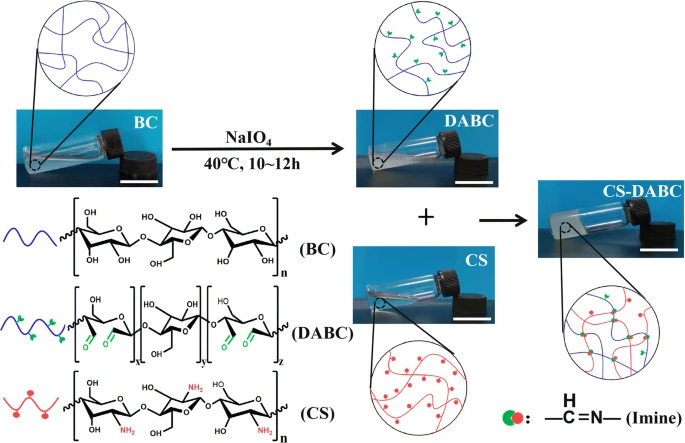
\includegraphics[width=0.7\linewidth]{Figures/CS_DABC_condensation.jpg}
    \caption{Schematic representation of hydrogel synthesis from chitosan and dialdehyde bacterial cellulose \autocite{liAllnaturalInjectableHydrogel2020}}
    \label{fig:CS_DABC_condensation}
\end{figure*}

The JTA combines several natural and synthetic materials, all of which must be safely broken down within the body to serve as an effective treatment. Alginate, a water-soluble polysaccharide which makes up the hydrophilic matrix of the hydrogel, degrades into monosaccharides, primarily guluronic and mannuronic acid units. These are very easily excreted from the body via the renal system. 
Chitosan, a cationic polymer typically used in the bioadhesive layer of the JTA, degrades into glucosamine and N-acetylglucosamine. These monosaccharides are involved in the body's natural metabolic processes, so they are very easily reintegrated into the body's metabolic system following the breakdown of the JTA \autocite{guarinoDegradationPropertiesMetabolic2015}.
Polyacrylamide, a synthetic polymer that makes up the backbone of the double-network structure, breaks down into acrylamide monomers. These synthetic byproducts can either be metabolized by the liver before being excreted via urine, or they can undergo conjugation with glutathione or glutathione-S-transferases, making them non-toxic and water-soluble \autocite{xiongPolyacrylamideDegradationIts2018}.
Schiff base linkages, which provide dynamic crosslinking within the JTA, hydrolyze into aldehydes and amines, which are non-toxic and easily metabolized or excreted \autocite{xuHydrogelsBasedSchiff2019}.

The degradation process roughly follows in the following order, from quickest to slowest degradation: alginate, chitosan, imine bonds, polyacrylamide. This order is very beneficial for the healing process. Alginate and chitosan, being natural components of the hydrogel, degrade quickly within the body, softening it slightly.
This both increases the permeability of the hydrogel, allowing cells and nutrients to enter and exit more efficiently, and encourages integration of the healing tissues with the hydrogel \autocite{RN4}.
Imine bonds provide the self-healing factor of the JTA, allowing it to recover from minor deformations and maintain structural integrity under movement. However, these bonds also degrade over time, after about 1--3 months, allowing more mechanical load to be gradually shifted from the hydrogel onto the recovering tissue \autocite{xuHydrogelsBasedSchiff2019}.
The polyacrylamide backbone, being a synthetic polymer, is the last to degrade within the body. This structure is critical in providing support to the tissue and must degrade approximately synchronously with the recovery time of the injury.

    % Towards a Self-Healing JTA
    % Section header command contained in the subfile
    % for better figure formatting

    \begin{figure*}[hb]
    \centering 
    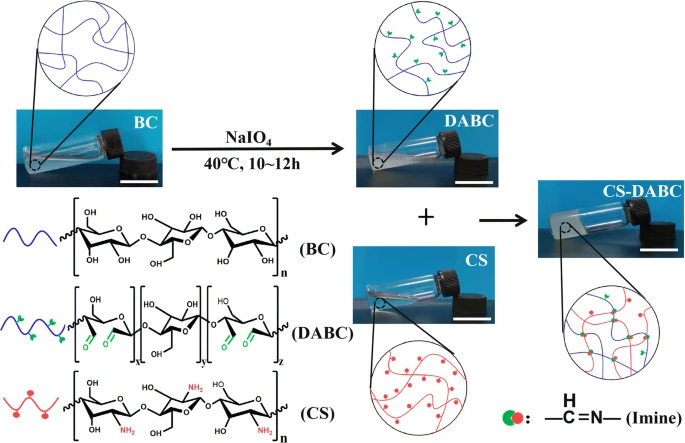
\includegraphics[width=0.7\linewidth]{Figures/CS_DABC_condensation.jpg}
    \caption{Schematic representation of hydrogel synthesis from chitosan and dialdehyde bacterial cellulose \autocite{liAllnaturalInjectableHydrogel2020}}
    \label{fig:CS_DABC_condensation}
\end{figure*}

\section{Towards a Self-Healing JTA}

A recent study by \citeauthor{liAllnaturalInjectableHydrogel2020} found that an all-natural, injectable hydrogel could be synthesized using chitosan and dialdehyde bacterial cellulose (\citeyear{liAllnaturalInjectableHydrogel2020}). This hydrogel uses imine bond dynamic cross-linkages to achieve its self-healing properties, where the Schiff base forms through the reaction of chitosan (as the amine) and bacterial cellulose (as the aldehyde).
The reaction can proceed under mild conditions (room temperature and pH = 7.2), and as it is all-natural, it has shown to be biocompatible. A schematic representation of this condensation reaction is given in Figure~\ref{fig:CS_DABC_condensation}.

Researchers tested the CS-DABC hydrogel's ability to self-repair after sustaining damage, a property that is desired for applications in wound dressings. To do so, round hydrogels were prepared and cut in half. One side was coloured orange, and the two half-discs were placed side-by-side in ambient conditions, as shown in Figure~\ref{fig:CS_DABC_self_healing}.
In just 3 hours, without external intervention, the two halves fused back together and reformed the original shape. They were also able to be picked up by one side, withstanding the force of gravity. Moreover, the gaps between the two hydrogel half-discs were observed under optical microscope.
The boundaries between the two sides were barely visible, demonstrating good self-healing properties from Schiff base reactions.

\begin{figure}[ht]
    \centering 
    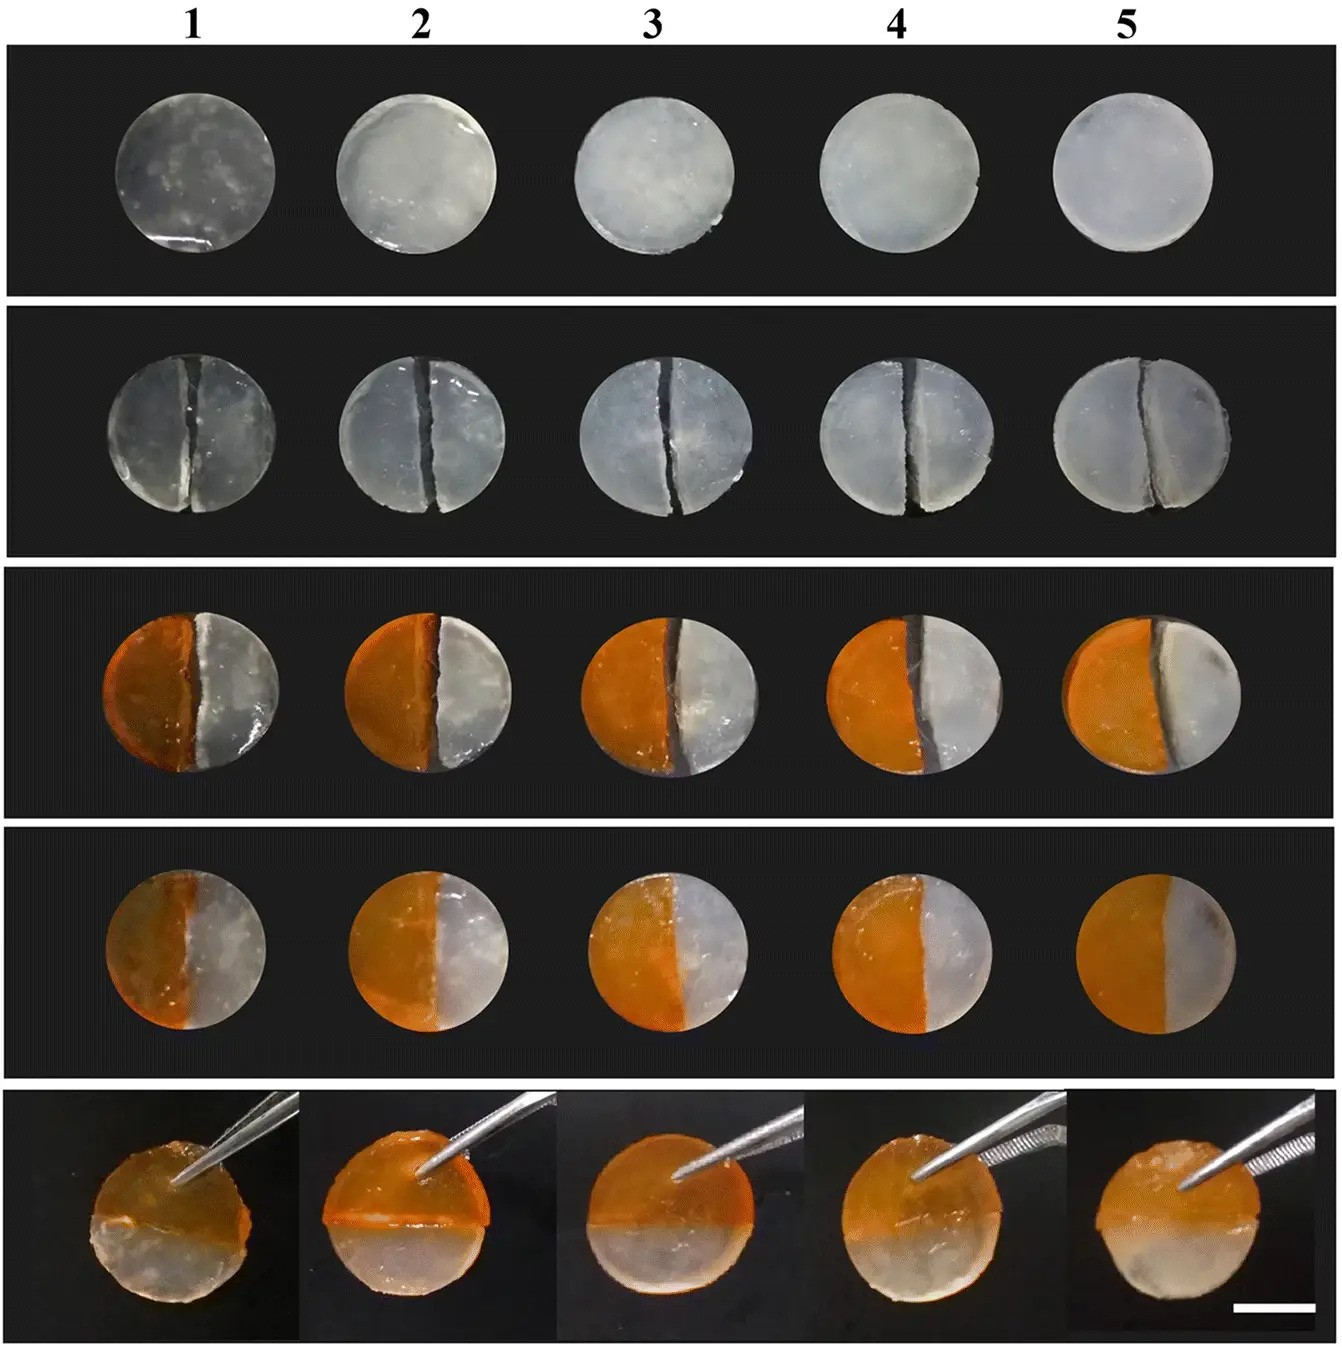
\includegraphics[width=\linewidth]{Figures/CS_DABC_self_healing.jpg}
    \caption{Self-healing properties of CS-DABC hydrogels. Discs were cut, stained, and healed under ambient conditions. [Adapted from \cite{liAllnaturalInjectableHydrogel2020}]}
    \label{fig:CS_DABC_self_healing}
\end{figure}

Additionally, the chitosan dressing exhibits antimicrobial properties, which reduces the risk of cross-contamination and promotes healthy healing of the wound. To evaluate these properties, the hydrogel was tested as an antibiotic against strains of \textit{E. coli} and \textit{S. aureus}.
Far fewer bacterial colonies were observed in the samples treated with CS-DABC compared to the control. As the hydrogel's protonated amino groups bind to the bacterial cell wall, effectively destroying it, bacterial growth is inhibited \autocite{liAllnaturalInjectableHydrogel2020}.

This self-healing hydrogel presents a promising application for tendon repair. Since JTAs already have a chitosan layer, it could be possible to synthesize Schiff bases directly on the existing structure using a similar technique as \citeauthor{liAllnaturalInjectableHydrogel2020}, leading to increased mechanical strength through the integration of self-healing properties.
% This self-healing hydrogel, therefore, has an interesting application for tendon repair. Given that JTAs have a chitosan side, it could be possible to augment their mechanical strength by integrating self-healing properties.

    \section{Methods of Testing Hydrogel Efficacy}

The efficacy of a hydrogel depends on several factors. Absorption, or swelling, tests,
approximated by placing the scaffold in a liquid medium and measuring the percentage increase
in weight. This serves as a measure of permeability, simulating the scaffold's ability to allow cells
and nutrients into the healing area. Stress-strain tests are used to approximate mechanical
strength, ensuring that the hydrogel will not collapse or overextend under mechanical stress.
Adhesion is measured via lap shear or peel tests \autocite{RN5}, which provide a numerical
measure for the ability of the hydrogel to resist movement after its placement. Degradation rate
can be measured in a couple ways, by measuring the overall weight of the scaffold at two or more
points in time. Degradation is measured as a percentage loss in mass or as a
percentage change in the diameter of individual fibrils that make up the matrix. These tests are
effective at measuring individual properties of the matrix ex vivo and predicting the success of
the hydrogel before it is used for treatment. However, an overall test can also be conductive
post-treatment, simply by measuring the strength of the tendon or ligament relative to its original
strength.

\subsection{Biocompatibility}

The Janus Tough Adhesive has shown to exhibit high biocompatibility during testing, despite it containing the synthetic polymer polyacrylamide. To evaluate their performance and impact on natural tissues, \citeauthor{freedmanEnhancedTendonHealing2022} (\citeyear{freedmanEnhancedTendonHealing2022}) experimentally tested  injured and healthy rats, and applied the JTA to the patellar tendon.
For three weeks, potential swelling of the tendon and degredation of the gel were assessed by high frequency ultrasound. When a tendon becomes injured, its echogenicity---the amount of sound it reflects---decreases, because its collagen fibres become more disorganised and less densely packed \autocite{hodgsonTendonLigamentImaging2012}.
Researchers also found that injured tendons without application of the JTA had larger cross-section areas, indicating increased swelling as shown in Figure~\ref{fig:JTA_Patellar_cross_section}. A decrease in inflammation in the affected tendon therefore suggests that the JTA was effective and well-tolerated by the body.
\begin{figure*}[ht]
    \centering
    \begin{minipage}[b]{0.45\textwidth}
        \centering
        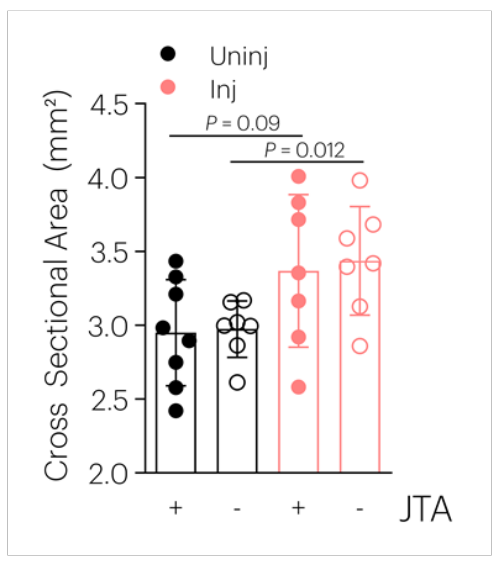
\includegraphics[width=0.6\linewidth]{JTA_cross_section.png}
        \caption{Patellar tendon cross-sectional area (mm\textsuperscript{2}) after 3 weeks of treatment [Adapted from \cite{freedmanEnhancedTendonHealing2022}]}
        \label{fig:JTA_Patellar_cross_section}
    \end{minipage}
    \hfill
    \begin{minipage}[b]{0.45\textwidth}
        \centering
        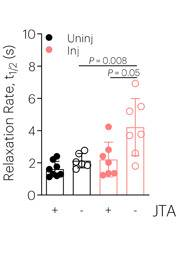
\includegraphics[width=0.6\linewidth]{Figures/JTA_relaxation_patellar.jpeg}
        \caption{Patellar tendon relaxation rate [Adapted from \cite{freedmanEnhancedTendonHealing2022}]}
        \label{fig:JTA_Patellar_relaxation}
    \end{minipage}
\end{figure*}

Furthermore, in the patellar tendon, the JTA was found to have improved tendon relaxation (Figure~\ref{fig:JTA_Patellar_relaxation}), without impacting natural properties such as elastic mechanics, dynamic modulus, or linear modulus.

% Biocompatibility of the JTA was also tested in more complex use cases, such as the rotator cuff and Achilles tendon. 

\subsection{\textit{In vivo} Testing Methods}

Hydrogels can be observed in vivo through various imaging methods including MRI, ultrasound,
and fluorescence. MRIs provide high-resolution contrast that allows researchers to observe
whether the hydrogel remains at the injury site. The swelling of the hydrogel and surrounding
tissues can also be monitored to ensure the hydrogel remains mechanically sound and the
surrounding tissue does not become irritated. Hydrogels are sometimes labeled with contrast
agents like gadolinium to make them more visible. Ultrasound imaging allows for both direct
imaging of the hydrogel and indirect imaging via the effect on adjacent structures. Ultrasound is
particularly beneficial in assessing adherence and in observing the effect of the hydrogel on joint
mobility. In the patellar tendon, the JTA was found to have improved tendon relaxation (Figure~\ref{fig:JTA_Patellar_relaxation}), without impacting natural properties such as elastic mechanics, dynamic modulus, or linear modulus. Fluorescence imaging uses fluorescent tags to track the movement of the hydrogel.
This makes it particularly effective in tracking hydrogel degradation and in visualizing
interactions with adjacent tissues. \citeauthor{freedmanEnhancedTendonHealing2022} showed the effectiveness of imaging
techniques in their rat experiments and also measured the effectiveness of the hydrogel on
recovery. The newly formed rat tendons were removed and tested, showing that the hydrogel
allowed the tendons to recover up to 80\% of their original strength, a marked improvement on
traditional surgical methods.

\subsection{\textit{Ex vivo} Testing Methods}

Ex vivo methods of testing are important to ensure the hydrogel will be effective when it is
placed in the body. Testing should ideally occur under wet conditions to simulate being in an
aqueous body environment. Absorption, or swelling, tests, approximated by placing the network
in a liquid medium and measuring the percentage increase in weight. This serves as a measure
of permeability, simulating the hydrogel's ability to allow cells and nutrients into the healing area.
An ideal hydrogel should fall between 100--500\%, indicating that it can swell enough to allow
cells and nutrients to enter without compromising structural integrity \autocite{zhangProtocolEfficientlyMeasuring2020}. Stress-strain
tests are used to approximate mechanical strength, ensuring that the hydrogel will not collapse
or overextend under mechanical stress. The ultimate tensile strength of the hydrogel should
approximately match the strength of the developing tendon, which falls between the range of
0.5--5 MPa. The Young's modulus of the hydrogel should also fall within a medium range of
about 0.1--10 MPa, ensuring that it remains flexible, while still providing appropriate support of
the tendon \autocite{xiaoMechanicalTestingHydrogels2013}. Adhesion is measured via lap shear or peel tests \autocite{ChenAdvancesApplicationHydrogel}, which
provide a numerical measure for the ability of the hydrogel to resist movement after its
placement. An adhesion strength of anywhere between 5--50 kPa is considered sufficient for
preventing detachment, but not so high to restrict motion or cause trauma. Degradation rate can
be measured in a couple ways, by measuring the overall weight of the scaffold at 2 or more
points in time and representing degradation as a percentage loss in mass or by measuring the
percentage change in the diameter of individual fibrils that make up the matrix. Ideally, the
hydrogel degrades approximately in sync with healing, about 10--30\% within the first month,
before gradually degrading over the next 6--12 months \autocite{zhuTailoringDegradationRates2015}. These tests are effective at
measuring individual properties of the matrix ex vivo and predicting the success of the hydrogel
before it is used for treatment.

    \section{Expected Outcomes}

    The proposed Janus Tough Adhesive hydrogel drug delivery system has a fracture energy of 9000~J/m\textsuperscript{2}, far higher than conventional hydrogels (100~J/m\textsuperscript{2}) and natural cartilage (1000~J/m\textsuperscript{2}), and on a similar scale a natural rubbers (10,000~J/m\textsuperscript{2}).
It uses imine bonding to dynamically re-form its cross-linkages should they fracture, increasing its lifespan.
The biomimetic adhesive has also shown adhesive strength exceeding 1000~J/m\textsuperscript{2}, and the reverse side mimics the friction generated by other biological tissues, allowing for natural tendon gliding.
Furthermore, the JTA has been shown to increase drug-loading capabilities 5000-fold when compared to current capacities (0.01--1~mg/mL). Drugs are released as the polymer network breaks down, which can be tuned to occur synchronously with healing.
The JTA's monomers are biocompatible and are metabolised by the liver or excreted by the body's urinary system.
As a result of its mechanical properties, drug-loading capabilities, and tuneable degradation rate, the proposed JTA drug delivery system is an ideal candidate for tendon repair applications. Altogether, it reduces the need for invasive treatments and accelerates recovery, leading to more effective, patient-friendly therapies for musculoskeletal injuries.

    \onecolumn
    \printbibliography
\end{document}